Ni la materia oscura ni la energía oscura sienten las fuerzas eléctricas y magnéticas y por tanto no interactúan con la luz, no la emiten ni la absorben. Son inmunes a las ondas electromagnéticas en todas las frecuencias, desde el radio, pasando por la luz visible hasta los rayos gamma, de forma rigurosa el calificativo oscuras no aplica, son transparentes, su existencia es supuesta por la interacción gravitatoria entre esta materia y las galaxias formadas por materia bariónica.


\subsection{Evidencias observacionales}

En la primera mitad del siglo pasado Paul Zwicky había estado observado agrupaciones de galaxias ligadas por atracción gravitatoria, siendo el primero en utilizar el \href{https://es.wikipedia.org/wiki/Teorema_del_virial}{Teorema de virial}. Del estudio de las velocidades radiales de ocho galaxias en el cúmulo Coma, Zwicky encontró una dispersión de velocidad inesperadamente grande $\sigma_{cz} = (1019 \pm 360) ~ \mathbf{km ~ s^{-1}}$ (recalculado en la actualidad por valor moderno $\sigma_{cz} = 1082 ~ \mathbf{km ~ s^{-1}}$ obtenido por \cite{colless_structure_1996}). Zwicky concluyó de estas observaciones que la densidad media del grupo Coma tendría que ser $\backsim 400$ (valor moderno recalculado de $\backsim 50$) veces mayor que la derivada de la materia luminosa (se sobreestimó la relación masa-luz del grupo Coma por asumir un parámetro de Hubble de $H_o = 558 ~ \mathbf{km ~ s^{-1} ~Mpc^{-1}}$ cuando su valor moderno de $H_o = 67.15~\mathbf{km~s^{-1} ~Mpc^{-1}}$), como conclusión de sus observaciones el mismo postula:

\begin{minipage}{0.9\linewidth}
\vspace{5pt}%margen superior de minipage
{\small }
\textit{``Si se confirma esta sobredensidad, llegaríamos a la sorprendente conclusión de que la materia oscura está presente en Coma con una densidad mucho mayor que la materia luminosa ... De estas consideraciones se deduce que la gran dispersión de velocidad en Coma representa un problema no resuelto''}
\begin{flushright}
presente en la referencia \cite{bergh_early_1999}
%(\citeauthor{Coulouris}, \citeyearNP{Coulouris}: 10)
\end{flushright}
\vspace{5pt}%margen inferior de la minipage
\end{minipage}

%\begin{figure}
%\centering
%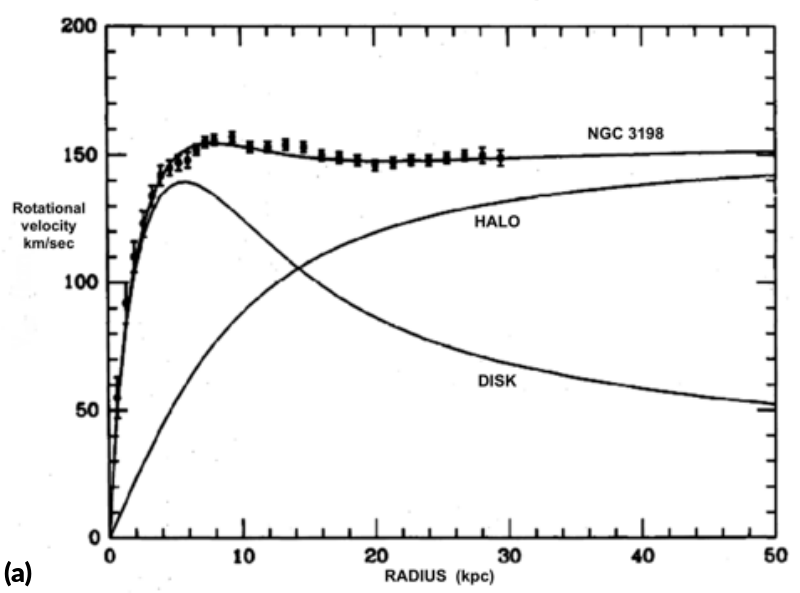
\includegraphics[width=0.49\textwidth]{Fisica_de_Particulas/imagenes/fritz.png}
%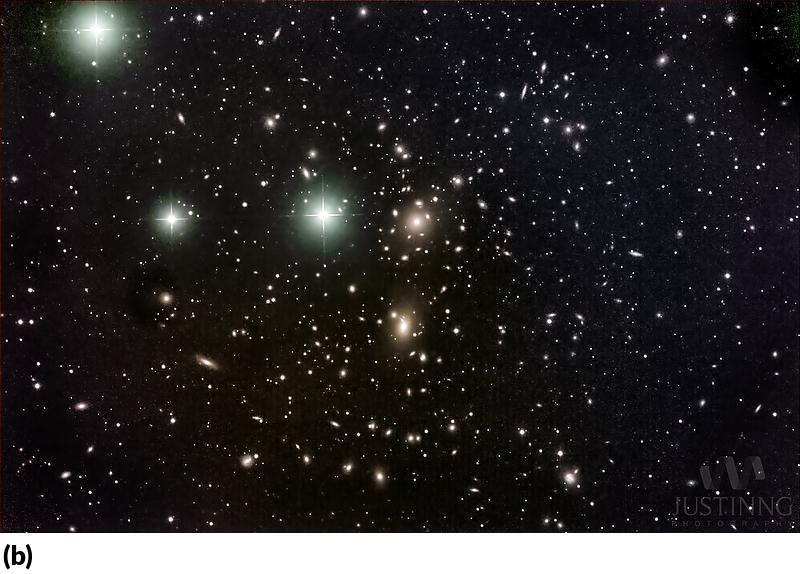
\includegraphics[width=0.49\textwidth]{Fisica_de_Particulas/imagenes/Coma-Cluster.jpg}
%\caption{(a) Gráficos de velocidad de rotación en función de la lejania del centro de la galaxia NGC 3198. Página de origen: \url{https://earthsky.org/clusters-nebulae-galaxies/the-coma-berenices-galaxy-cluster}, (b) Visualización del cúmulo de $\backsim 10^4$ galaxias Coma. Página de origen: \url{https://earthsky.org/clusters-nebulae-galaxies/the-coma-berenices-galaxy-cluster}}
%\label{coma}
%\end{figure}
%Esta cuestión continuo siendo un enigma hasta que Vera Rubin y Kent Ford confirmaron la prueba de su existencia en 1970 al trazar la curva de rotación de la galaxia ver el gráfico correspondiente a la Fig. \ref{coma}a para \href{https://en.wikipedia.org/wiki/NGC_3198}{NGC 3198} (es una galaxia espiral en la constelación de la Osa Mayor) muestra que la velocidad de la materia visible es esencialmente constante aunque nos elejemos del centro para distancias mayores de $\gtrsim 5 ~kpc$ desde el centro de la galaxia, en lugar de tener una caída Kepleriana proporcional a $1/r$. 

y con ello nace la primera mención de materia oscura en el ámbito científico moderno. En la actualidad se continuan los intentos por comprender el problema galáctico de la masa visible faltante, ejemplos se pueden encontrar proyectos de simulaciones \citep{deur_relativistic_2020, wu_galactic_2015} o mediante la comparacion empírica con los datos experimentales \cite{mielke_dark_2006}, con altos niveles de predicción.

%\subsubsection{Lentes gravitacionales}
Otra evidencia viene de las \href{https://en.wikipedia.org/wiki/Gravitational_lens}{lentes gravitacionales} (Fig. \ref{lentes}). La gravedad afecta a todo el espectro de ondas electromagnéticas, incluyendo radio, infrarrojos, luz visible y ultravioleta, siendo el grado de desviación mayor mientras mayor sea la masa que actúa como lente gravitacional, siento esta predicción unos de los mayores resultados de Einstein, en estos cálculos se pudo evidenciar el efecto para cálcular el valor de masas de grandes cúmulos midiendo las desviaciones de la luz.

\begin{figure}[htbp]
\centering
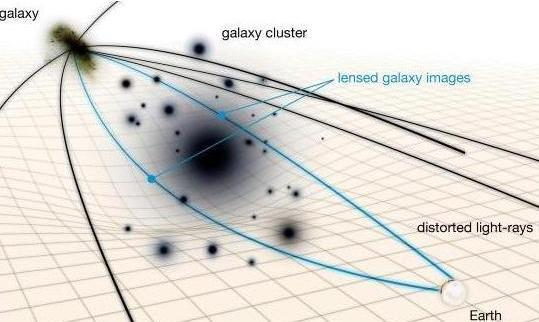
\includegraphics[width=.6\textwidth]{Cap1/imagenes/lentes.jpg}
\caption[Diagrama de cúmulo de galaxias que actúa como lente gravitatoria para una galaxia muy distante.]{Diagrama de cúmulo de galaxias que actúa como lente gravitatoria para una galaxia muy distante.\footnotemark}
\label{lentes}
\end{figure}

\footnotetext{Página de origen: 
\href{https://alquimiayciencias.blogspot.com/2013/06/explicando-la-materia-oscura-cualquiera.html}{https://alquimiayciencias.blogspot.com/}}


Dadas sus características los \href{https://curiosoando.com/introduccion-a-las-lentes-gravitacionales}{lentes gravitacionales} son un importante herramienta para detectar la materia oscura, resultado de la comparación de lo resultados experimentales con los resultados de la relatividad general que predice la dinámica dependiente de la masa visible.

%En algunos casos, la lente no es lo suficientemente fuerte como para formar múltiples imágenes o arcos, sin embargo, la fuente aún está distorsionada porque es un hecho que hay algo de materia oscura entre nosotros y cada galaxia distante que vemos, %de aca que todas las galaxias tienen lentes, incluso si son solo un poco, 
%aquellas alteradas solo en una cantidad muy pequeña son llamadas lentes gravitacionales débiles.
%\begin{figure}[h]
%\centering
%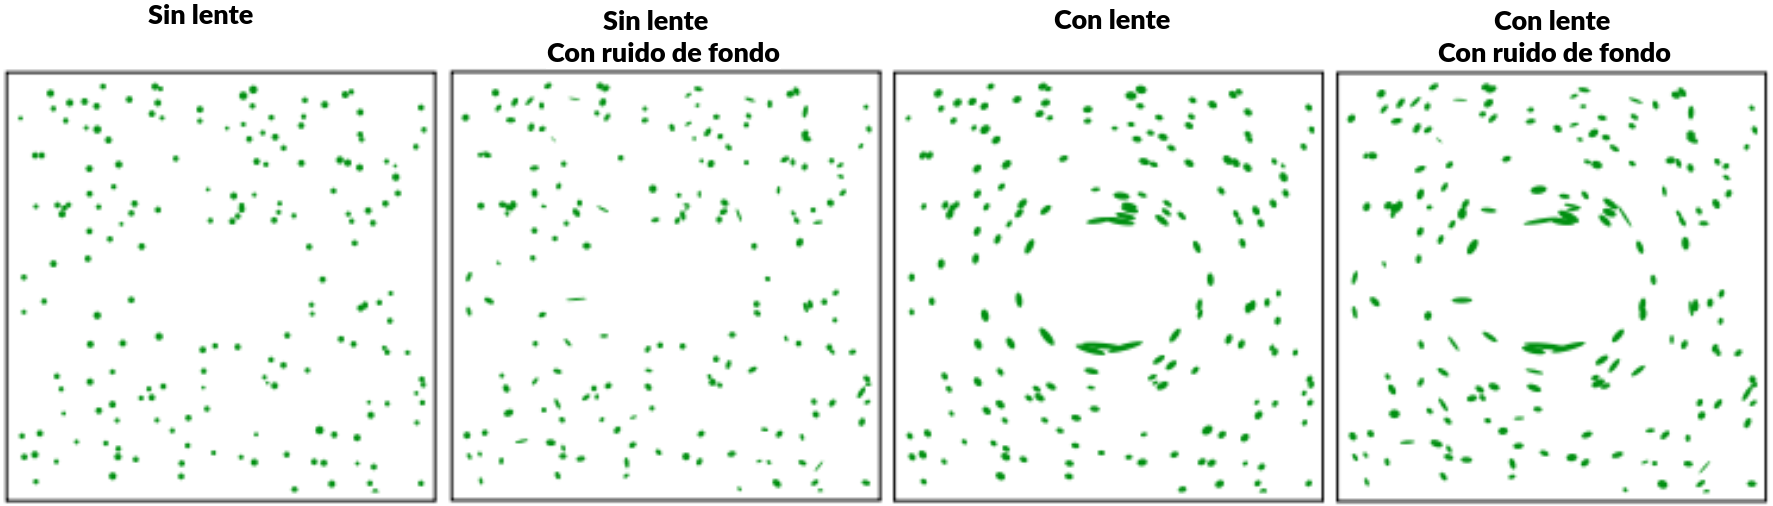
\includegraphics[width=1\textwidth]{Fisica_de_Particulas/imagenes/lentes.png}
%\caption{Simulación de un campo de galaxias circulares, el ruido de fondo es un grupo de galaxias realista de fondo. Página de origen: \url{https://fos.cmb.ac.lk/blog/gravitational-lensing-wonders-universe-iii/}}
%\label{lentes2}
%\end{figure}
%Nunca podemos ver esta modificación de forma con nuestros propios ojos en una imagen porque es demasiado pequeña, en vez de eso podemos calcular el efecto de lente promedio en un conjunto de galaxias, normalmente bajo suposiciones (ver Fig. \ref{lentes2}), como considerar que todas las galaxias tienen una formas elípticas o que están orientadas al azar en el cielo, estas se traten de forma estadística.

%Trabajos dedicados a la simulación numérica (ver referencia \citep{munshi_statistics_2001, fosalba_mice_2015}) para conocer los efectos de la distribución de la materia oscura en un el universo (ver Fig. \ref{lentes3}), las trayectorias de los rayos se desvían evidentemente por los efectos gravitacionales de la materia provocando que las galaxias esten ligeramente alargadas en una dirección común determinada por la distribución de la materia oscura a lo largo de esa línea de visión particular, ya que la distorsión es muy pequeña, esta requiere un tratamiento estadístico cuidadoso en muchos parches en el cielo.
%\begin{figure}[h]
%\centering
%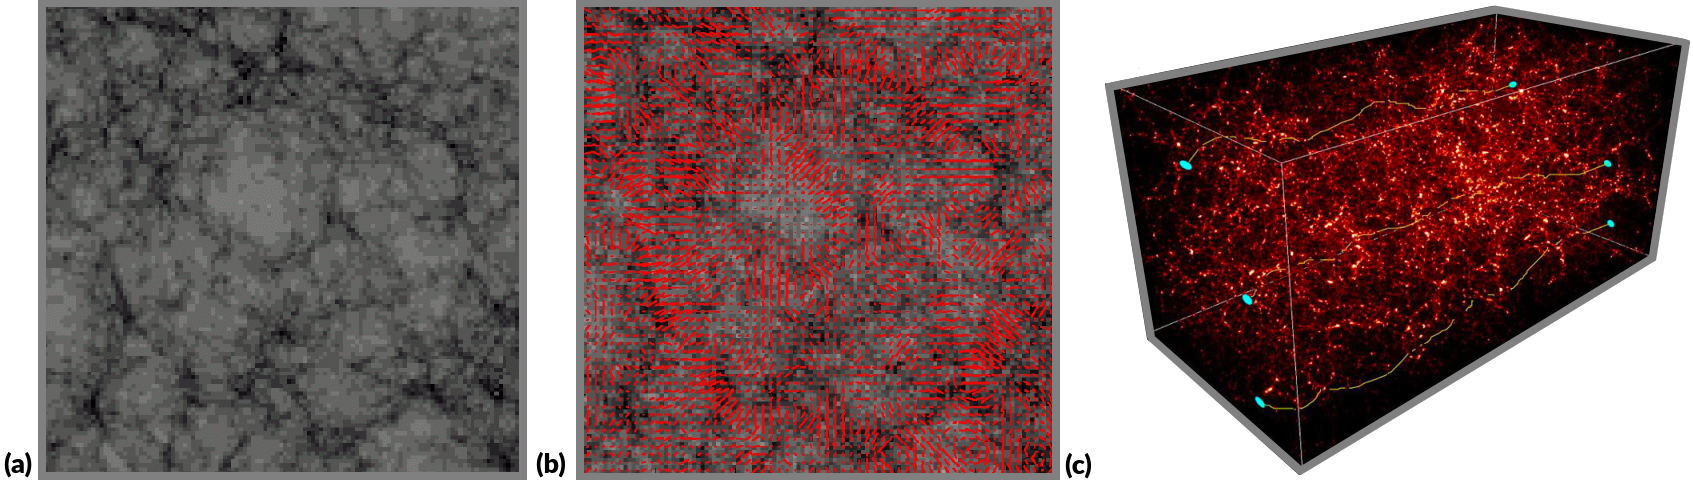
\includegraphics[width=1\textwidth]{Fisica_de_Particulas/imagenes/lentes3.png}
%\caption{(a) Simulación computacional de materia oscura, (b) Efecto lente gravitación, (c) Simulación numérica que muestra la distribución de la materia oscura en un gran volumen del universo,  los tres discos azules representan tres galaxias distantes, Las líneas que cruzan la caja representan rayos de luz de esas galaxias que se propagan a través del universo. Página de origen: \url{http://www.cfht.hawaii.edu/News/Lensing/index.html\#ST}}
%\label{lentes3}
%\end{figure}
%Las lentes gravitacionales fuertes se caracterizan por la curvada distorsión observada de las galaxias de fondo, estas han sido observada alrededor de un cúmulo poco distante como el Abell 1689 o 3827. %(ver Fig. \ref{lentes}b). Midiendo la distorsión geométrica, se puede obtener la masa del cúmulo que causa el fenómeno. Estas lentes permiten ver objetos distantes, sobre todo galaxias lejanas, al intensificar su luz, motivo por el cual su estudio es motivo de investigación (\cite{schafer_lenstool-hpc_2020}). Al observar la luz de las galaxias más distantes, algunas tan antiguas que su formación se remonta a las primeras fases de expansión del Universo, los astrónomos pueden estudiar las condiciones de hace miles de millones de años, e incluso que sucedía durante la formación de estas galaxias, de forma que pueden ser aplicadas de modo similar a los telescopios. Un caso especial de estos lentes son los \href{https://en.wikipedia.org/wiki/Einstein_ring}{anillos de Einstein}, causada por la alineación exacta de la fuente, la lente y el observador, este fue predicho por este en 1912.

%Las microlentes se suelen formar por el paso de una estrella o planeta delante de otra estrella u otro objeto más lejano. La luz del objeto distante no está tan distorsionada como en las lentes fuertes, ni siquiera alcanza a la distorsión de las lentes débiles; la distorsión de la imagen puede ser prácticamente imperceptible, pero la disminución en la intensidad de la luz pone de manifiesto las microlentes. Gracias a las microlentes se han descubierto numerosos planetas extrasolares.
\begin{figure}[htbp]
\centering
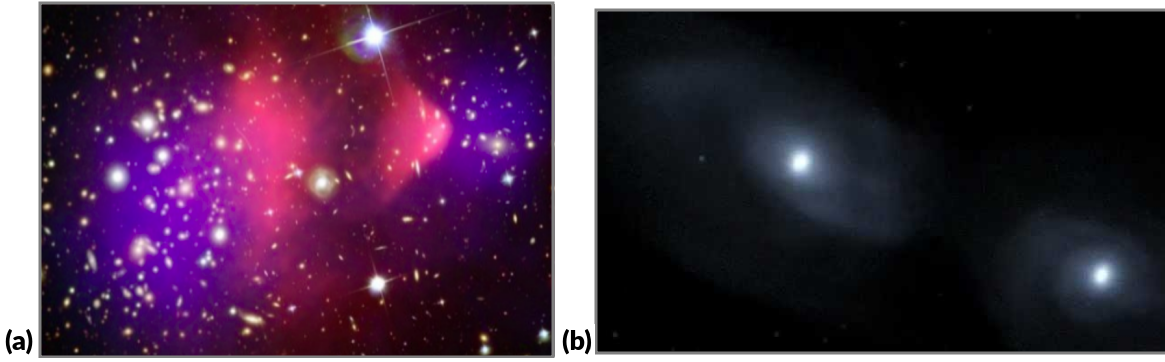
\includegraphics[width=.9\textwidth]{Cap1/imagenes/fritz2.png}
\caption[(a) Coalisión de dos cúmulos de galaxias 1E 0657-56 conocida como \href{https://en.wikipedia.org/wiki/Bullet_Cluster}{cúmulo bala}.
, (b) Simulación por computadora de la futura colisión prevista de las dos galaxias más grandes del Grupo Local, Andrómeda (M31) y la Vía Láctea. ]{
(a) Coalisión de dos cúmulos de galaxias 1E 0657-56 conocida como \href{https://en.wikipedia.org/wiki/Bullet_Cluster}{cúmulo bala}.
, (b) Simulación por computadora de la futura colisión prevista de las dos galaxias más grandes del Grupo Local, Andrómeda (M31) y la Vía Láctea. \footnotemark }
\label{coalision}
\end{figure}
 
\footnotetext{Página de origen: (a) \href{https://en.wikipedia.org/wiki/Bullet_Cluster\#/media/File:1e0657\_scale.jpg}{https://en.wikipedia.org/wiki/Bullet\_Cluster\#/media/File:1e0657\_scale.jpg} \\
. ~~~~~~~~~~~~~~~~~~~~~~~~~~~~~~~~~~~~ (b) \href{https://hubblesite.org/contents/media/videos/2012/20/700-Video.html?news=true}{https://hubblesite.org/contents/media/videos/2012/20/700-Video.html?news=true}}

%\subsubsection{Coalisión de galaxias}
Resultado de las observaciones realizadas por el Chandra de rayos $X$ de la NASA y el Telescopio Espacial Hubble al estudiar el grupo MACSJ0025.4-1222, se realizó el seguimiento de la colisión de dos cúmulos de galaxias (ver Fig. \ref{coalision}a), en este se detecta como la temperatura de la materia bariónica aumenta y esta se emiten rayos X. Siendo las áreas azules de la Fig. \ref{coalision} un mapa reconstruido de la materia oscura hecha mediante el uso de lentes gravitacionales, la materia bariónica se muestra en rosa mostrándose separada de la mayoría de la materia que comprende los grupos que se muestran en azul \citep{marsh_strings_2019}.




%Dada la riqueza en el fenómeno de coalisión este es ampliamente estudiado incluso en la actualidad en el 2018 la \textbf{UNAM} (Universidad Nacional Autónoma de México) diseñó el \textbf{NEFER} (Nuevo Espectrómetro Fabry-Perot de Extrema Resolución), invento integrable al espectrómetro \textbf{OSIRIS} del Gran Telescopio Canarias (GTC) en España, permitiendo observar en dos dimensiones de alta resolución la formación estelar que se produce en las galaxias e inclusive la distribución de la materia oscura, todo mediente mapas bidimensionales de intensidades y velocidades de objetos astronómicos extendidos, diseñado principalmente para observar la emisión y las velocidades del medio interestelar de nuestra galaxia y de galaxias externas.

%La complejidad de estos fenómenos esta siendo arduamente estudiada, bajo la apuesta de que nuestra comprensión del mundo mejorara por ello, razón por lo cual los trabajos en esa linea son tema actual implementando continuamente la simulación como herramienta de análisis, este fue el caso de dos galaxias Andrómeda (M31) y la Vía Láctea, las cuales formaron parte de un arduo trabajo basada su predicción en mediciones con el telescopio espacial Hubble del movimiento adecuado de M31 en el cielo, junto con el desplazamiento al rojo de M31 (ver Fig. \ref{coalision})c relacionado con la referencia \cite{van_der_marel_m31_2012}. 
%Mientras previas investigaciones afirman la necesidad de incluir la materia oscura en las simulaciones hay que considerar algunas investigaciones que bajo el excepticismo de la existencia de materia oscura intenta encontrar otras fuentes de incertidumbre, posibles soluciones como sos presentados en la referencia \cite{bilek_mond_2018}, donde se intentan adaptar la relatividad general bajo un nuevo enfoque dada por la teoría \href{https://en.wikipedia.org/wiki/Modified_Newtonian_dynamics}{\textbf{MOND}} (del inglés \href{https://en.wikipedia.org/wiki/Modified_Newtonian_dynamics}{Modified Newtonian dynamics}) dando resultados que hacen cuestionar que tan cerca estamos de entender la materia oscura o su existencia.


%\subsubsection{Formación de estructuras}

%En las simulaciones la inclusión de la materia oscura es fundamental para explicar la formación de estructuras cosmologicas ya que la materia normal sucumbe a la fuerza de atracción de la materia oscura formando galaxias y cúmulos de ellas, por otro lado la energía oscura es cualquier entidad que haga que la expansión del universo se acelere.

En las investigaciones del proceso evolutivo del universo se hace necesario tener en cuenta la presencia de la materia oscura que frena la aceleración de la expansión y la energía oscura que lo acelera. Se hace necesario para los modelos cosmológicos del Big Bang considerar la presencia de los elementos oscuros para que exista correspondencia con las medidas de los parámetros asociados con la métrica \href{https://es.wikipedia.org/wiki/M\%C3\%A9trica_de_Friedman-Lema\%C3\%AEtre-Robertson-Walker}{\textbf{FLRW}} (\textbf{F}riedmann-\textbf{L}emaître-\textbf{R}obertson-\textbf{W}alker) de la relatividad general. 

%Las anisotropías del \CMB ~ se corresponden a una cosmología donde gran parte de la materia interactúa con los fotones de forma más débil que las fuerzas fundamentales conocidas que acoplan las interacciones de la luz con la materia bariónica. Así mismo, se necesita una cantidad significativa de materia fría no-barionica para explicar la estructura a gran escala del universo. %Las observaciones sugieren que la formación de estructuras en el Universo procede jerárquicamente, con las estructuras más pequeñas uniéndose hasta formar galaxias y después cúmulos de galaxias. 
%Según se unen las estructuras en la evolución del Universo, empiezan a "brillar" ya que la materia bariónca se calienta a través de la contracción gravitacional y los objetos se aproximan al equilibrio hidrostático. La materia barionica ordinaria tendría una temperatura demasiado alta y demasiada presión liberada desde el Big Bang para colapsar y formar estructuras más pequeñas, como estrellas, a través de la inestabilidad de Jeans. La materia oscura actúa como un compactador de estructuras. %Este modelo no sólo se corresponde con investigaciones estadísticas de la estructura visible en el Universo sino también se corresponden de forma precisa con las predicciones de materia oscura de la \WMAP.

%Para obtener el inverso de formación de estructuras necesita algún tipo de la materia oscura para funcionar. Se han utilizado simulaciones por ordenador de miles de millones de partículas de materia oscura para confirmar que el modelo de materia oscura fría de la formación de estructuras es consistente con las estructuras observadas en el Universo mediante las observaciones de galaxias, como la Sloan Digital Sky Survey y la 2dF Galaxy Redshift Survey, así como las observaciones del bosque Lyman-alfa. Estos estudios han sido cruciales en la construcción del modelo Lambda-CDM que mide los parámetros cosmológicos, incluyendo la parte del Universo formada por bariones y la materia oscura.


%Entre sus observaciones de los experimentos más recientes (ver Anexo \ref{anexoA}) se ha reportado un flujo de positrones anómalo que tiene una posible explicación en el proceso de aniquilación de partículas de materia oscura, donde se libera energía en forma de positrones. Dicho flujo anómalo puede observarse
%a partir de los 25 $\mathbf{GeV}$ en la Figura \ref{fig:AMS_positronflux} donde también se presenta una comparación con otros experimentos que observan similar comportamiento.
%
%\begin{figure}[htbp]
%    \centering
%    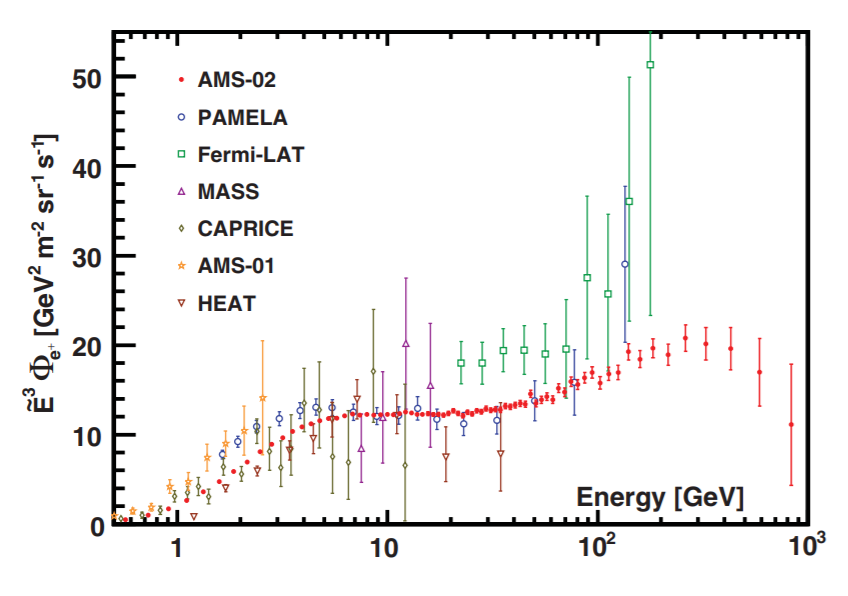
\includegraphics[width=0.75\textwidth]{Fisica_de_Particulas/imagenes/AMS_positronflux.png}
%    \caption{Flujo de positrones medido por el experimento AMS-02, comparado con los experimentos PAMELA, Fermi-LAT, MASS, CAPIRCE, AMS-01 y HEAT.}
%    \label{fig:AMS_positronflux}
%\end{figure}

Estos resultados cosmológicos han motivado a los físicos teóricos de altas energías a postular nuevos modelos en los cuales la composición de la materia oscura se pueda entender por medio de nuevas partículas elementales no descritas en el modelo estándar y que sin embargo podrían estar siendo producidas en los aceleradores de partículas modernos como el Gran Colisionador de Hadrones en Ginebra, Suiza. Los modelos propuestos se encuentran en la categoría que se conoce como extensiones al modelo estándar y por lo general involucran la existencia de nuevas partículas cuyas fuerzas e interacciones están descritas por alguna variación de la teoría cuántica de campo, lo que sugiere que sus mecanismos de producción y propiedades pueden ser estudiados por el formalismo de la física de partículas y la parte experimental por medio de los detectores de partículas con métodos de recolección de datos, selección de eventos y técnicas estadísticas para el análisis y extracción de posibles señales.




\subsection{Composición de la materia oscura}
%La existencia de la materia oscura es respaldada por muchos fenómenos cosmológicos, de aquí que los investigadores teoricen sobre su composición.

%\subsubsection{Materia oscura bariónica }
En los primeros a\~nos de estudio del problema de la materia oscura en el Universo, se propuso que esta podría ser materia bariónica y otras partículas ligadas a ellos en forma de objetos compactos masivos pero con una emisión electromagnética muy débil. Entre estos candidatos a materia oscura bariónica se encuentran los gases no luminosos, los objetos compactos y masivos de los halos galácticos (MACHOs) y las enanas marrones, sin embargo, múltiples líneas de evidencia contradicen este hecho, ya que contribuyen muy poco a la densidad crítica del Universo.
%La cantidad total de materia oscura bariónica puede ser calculada a partir de la nucleosíntesis del big bang, y las observaciones del fondo de microondas cósmicas. Ambas indican que la cantidad de esta materia es mucho menor que la cantidad total de materia oscura.
%En el caso de la nucleosíntesis, el problema es que una gran cantidad de materia normal significa un universo joven muy denso, es decir, una conversión eficiente de materia a helio-4 y menos deuterio restante. Si asumimos que toda la materia oscura del universo está formada por bariones, entonces hay muchísimo más deuterio en el universo. Esto puede resolverse si hubiera alguna manera de generar deuterio.
%pero se han realizado grandes esfuerzos desde los años 70 con resultado negativo, generalizando la idea de que no puede crearse dicho elemento.

%\subsubsection{Materia oscura no-bariónica} 
Entonces ante la propuesta de que la materia oscura puede estar compuesta por materia no bariónica, esta se puede clasificar en caliente, tibia o fría. Esta clasificación está relacionada con la dispersión de velocidades de la partícula en el momento en que se desacopló del plasma primigenio:
\begin{itemize_f}
\item \textbf{Materia oscura caliente: } aquellas que se mueven \href{https://en.wikipedia.org/wiki/Ultrarelativistic_limit}{ultrarrelativistamente}. Estas hacen referencia a una determinada partícula $\chi$ de masa $m_\chi$ con una velocidad relativista al momento de desacoplarse del plasma primigenio, por lo tanto, su temperatura cumple con la condición $T_\chi \gg m_\chi$. 

\item \textbf{Materia oscura fría :} aquella que no se mueven relativistamente al momento de desacoplarse ($v_\chi \sim 0$), por lo cual $T_\chi \ll m_\chi$. 

\item \textbf{Materia oscura templada o tibia :} aquella que se mueven relativistamente. %ella posee características intermedias entre las frías y calientes, o sea, con dispersión de velocidades al momento de desacoplarse mayores a las de la materia oscura fría pero menores a las de la materia oscura caliente.
\end{itemize_f}

Algunos de los candidatos a materia oscura más populares en el área de la física de partículas son: 

\begin{itemize}
\item \textbf{\Axiones}%\footnote{Más información en: \href{https://wikimili.com/en/Axion}{https://wikimili.com/en/Axion}} 
: Esta partícula es el bosón pseudo-Goldstone que resulta del rompimiento espontáneo de la simetría Peccei-Quinn, \citep{axion_2019}. Esta simetría se postula en 1977 en las extensiones del modelo estándar para resolver el problema de la violación carga-paridad \textbf{CP}\footnote{Se basa en la composición de la simetría \textbf{C} y la simetría \textbf{P}, la primera afirma que las leyes de la Física son invariantes  ante cambios de partículas de carga positiva a negativa y la segunda postula que la invarianza bajo inversiones especulares. } de la interacción fuerte en \QCD. Las observaciones cosmológicas y las mediciones en los aceleradores de partículas acotan la masa del axión a valores de $\lesssim 10^{-2}~\mathbf{eV}$ por lo que cae en la categoría de materia oscura fría. Una de las características de los axiones es que dado que tiene interacciones extremadamente débiles con otras partículas, éstas podrían no estar en equilibrio térmico en el Universo temprano. 

\item \WIMPs ( \textbf{W}eakly \textbf{I}nteracting \textbf{M}assive \textbf{P}articles) %\footnote{Más información en: \href{https://wikimili.com/en/Weakly\_interacting\_massive\_particles}{https://wikimili.com/en/Weakly\_interacting\_massive\_particles}}
: son partículas que se desacoplan siendo no relativistas cuando el Universo tenía una temperatura de $\simeq 1~ GeV$, por lo que caen en la clasificación de materia oscura fría, \citep{wimps_2018}. Las masas
de los \WIMPs ~ abarcan un intervalo de $10 ~ \mathbf{GeV} ~ - ~ 1 ~ \mathbf{TeV}$. Como su nombre lo indica, es un partícula que interactúa débilmente y gravitacionalmente con el resto de las especies del modelo estándar. 



Entre los candidatos se encuentran:
\begin{itemize}
\item 	\LSP (\textbf{L}ightest \textbf{S}upersymmetric \textbf{P}article)%\footnote{Más información en: \href{https://en.wikipedia.org/wiki/Lightest\_supersymmetric\_particle}{https://en.wikipedia.org/wiki/Lightest\_supersymmetric\_particle}}
: es el nombre genérico dado a la más ligera de las partículas hipotéticas adicionales que se encuentran en los modelos supersimétricos. En modelos con conservación de \href{https://es.wikipedia.org/wiki/Paridad\_R}{paridad R}\footnote{{Más información en: \href{https://es.wikipedia.org/wiki/Paridad\_R}{https://es.wikipedia.org/wiki/Paridad\_R}}}, el \LSP ~ es estable; en otras palabras, el \LSP ~ no puede descomponerse en ninguna partícula del \ME~ ya que poseen paridad R opuesta. Algunos ejemplos más conocidos son el sneutrino ligero, el neutralino ligero y el gravitonio.

%Más información en: \href{https://en.wikipedia.org/wiki/Lightest_supersymmetric_particle}{\texttt{https://en.wikipedia.org/wiki/Ligh\-test\_su\-per\-symme\-tric\-\_\-par\-ti\-cle}}.

\item \href{https://en.wikipedia.org/wiki/Kaluza\%E2\%80\%93Klein_theory}{\textbf{LKP} (\textbf{L}ightest {K}aluza-Klein \textbf{P}article) :} son las partículas hipotéticas que cumplen con la teoría de \href{https://en.wikipedia.org/wiki/Kaluza\%E2\%80\%93Klein_theory}{Kaluza-Klein (teoría \textbf{KK})} unificadora de la gravitación y electromagnetismo construida alrededor de la idea de una quinta dimensión más allá de los cuatro habituales del espacio y el tiempo, siendo considerada precursor de la teoría de cuerdas. Algunos de sus candidatos ligeros son el fotón \href{https://en.wikipedia.org/wiki/Kaluza\%E2\%80\%93Klein_theory}{\textbf{KK}} y el neutrino \href{https://en.wikipedia.org/wiki/Kaluza\%E2\%80\%93Klein_theory}{\textbf{KK}}, con masas en la escala $\mathbf{TeV}$ (para mas información, ver referencia \cite{servant_is_2003}).

%\item \textbf{LTP} (\textbf{L}ightest \textbf{T}-odd \textbf{P}article) :
\end{itemize}
\item \href{https://es.scribd.com/document/273103231/Dark-Pion-Particles-May-Explain-Universe-s-Invisible-Matter}{\textbf{SIMPs} (\textbf{S}trongly \textbf{I}nteracting \textbf{M}assive \textbf{P}article\textbf{s}) :} se supone que los piones oscuros interactúan mucho más fuertemente entre sí, se sugiere que en el universo primitivo los piones oscuros habrían chocado entre sí, reduciendo la cantidad de materia oscura, pero a medida que el universo se expande, las partículas colisionarían cada vez con menos frecuencia, hasta ahora, cuando se extienden de manera tan delgada que casi nunca se encuentran. En la nueva hipótesis, los piones de materia oscura están formados por quark de materia oscura que se mantienen unidos por gluones de materia oscura. (Los quarks ordinarios están unidos por gluones normales), en esta propuesta el gluón oscuro tendría masa, \citep{simps_2019}.

\item  \SUSY (\textbf{SU}per\textbf{SY}mmetry): postula la existencia de partículas supersimétricas compañeras al \ME, pero con espín diferente, \citep{susy_2020}. Esta se presenta como una simetría de tipo espacio-temporal. Una extensión supersimétrica del \ME ~ resuelve los principales problemas de jerarquía dentro de la teoría.
\end{itemize}

Las partículas supersimetrías son los candidatos más populares para la física de partículas no descubiertas. Esta supersimetría hipotética relaciona las propiedades de los bosones y los fermiones, y a pero a pesar de estar por ser verificada experimentalmente, es parte fundamental de muchos modelos teóricos. 
\begin{figure}[!b]
\centering
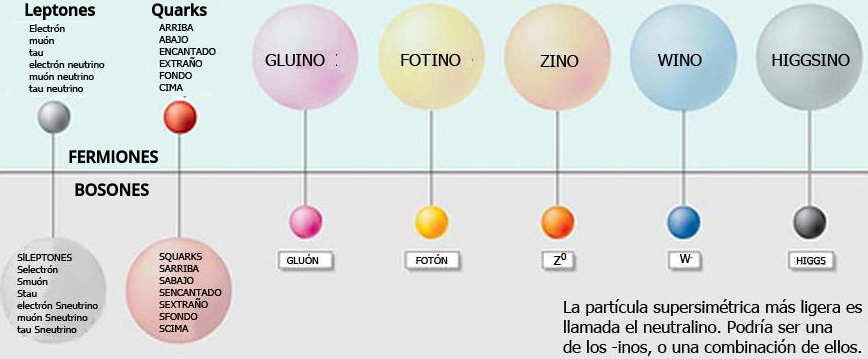
\includegraphics[width=.95\textwidth]{Cap2/imagenes/supersimetrias.png}
\caption{Extensión del Modelo Estándar bajo la existencia de la supersimetría (\SUSY). %Página de origen : \href{http://www.cienciakanija.com/2009/11/13/confiamos-en-susy-lo-que-realmente-busca-el-lhc/}{\texttt{http://\-www.cienciakanija.com/\-2009/\-11/13/\-con\-fia\-mos-\-en-\-susy-\-lo-\-que-\-real\-men\-te-bus\-ca-el-lhc/}}.
}
\label{susy}
\end{figure}

De forma general el \ME ~se construye a partir de simetrías fundamentales que dan lugar a leyes de conservación. En el caso de \SUSY, esta incluye todas las simetrías que ya contiene el \ME~ y añade otra más que involucra al espín. Esta teoría postula que a cada partícula del \ME ~le corresponde un compañero supersimétrico que tiene el espín contrario, de modo que, por cada fermión, \SUSY ~añade un bosón y por cada bosón se añade un fermión. Por tanto, el número de partículas predichas es el doble que en el \ME, como se visualiza en la Figura~\ref{susy}. %Los generadores $\mathbf{Q}$ son los tensores de transformación que actúan como:
%\begin{equation}
%\mathbf{Q}|\mathbf{Fermion}> ~ = ~ |\mathbf{Boson}> ~~~~ \textsf{y} ~~~~ \mathbf{Q}|\mathbf{Boson}> ~ = ~ |\mathbf{Fermion}>
%\end{equation}
%Desde su propia definición, este operador tiene dos propiedades de gran alcance:
%\begin{itemize}
%\item Cambia el spin de una partícula y como resultado sus propiedades espacio-temporales. Es por eso que la supersimetría no es una simetría interna sino una simetría de espacio-tiempo.
%\item En una teoría donde se realiza la supersimetría, cada estado de una partícula tiene al menos un supercompañero. Por lo tanto, en un entorno \SUSY, en lugar de estados de partículas individuales, uno tiene que lidiar con (super) múltiplos de estados de partículas.
%\end{itemize}

%Se espera que \SUSY ~puede dar solución al problema de la materia oscura mediante su teorizada relación con la materia del \ME, en la mayoría de modelos de supersimetría, la partícula supersimétrica más ligera o \LSP ~es necesariamente neutra y estable. %Esto significa que nuestro Universo estaría lleno de estas partículas masivas, neutras y estables, que por tanto serían buenas candidatas a formar la materia oscura.
Debido a que dichas compañeras supersimétricas aún no han podido ser creadas en el laboratorio, sus masas deben ser mucho mayores que las de las partículas originales. %Implicando entonces que la supersimetría, de ser cierta, está rota por algún mecanismo, 
La especificación de dicho mecanismo da lugar al Modelo Mínimo Estándar Supersimétrico \MSSM~(\textbf{M}inimal \textbf{S}upersymmetric \textbf{S}tandard \textbf{M}odel), que intenta explicar el problema de la materia oscura del universo, \citep{MSSM_1, MSSM_2}.




\subsection{Extensión del Modelo Estándar con Supersimetría}
 


%En el año 1973 por Julius Wess y Bruno Zumino presentan un modelo en la física de partículas el cual es conocido con el nombre de Modelo de Wess-Zumino, este es un modelo mínimo supersimétrico con solo un fermión y su súper compañero bosón. A pesar de que el modelo de Wess-Zumino no representa un modelo físico real, sirvió para fundamentar ciertos aspectos de los modelos físicos supersimétricos teorizados. 

%Entre las posibles búsquedas para descifrar la composición de la materia oscura, algunas de las más populares son entre las partículas 

El primer modelo supersimétrico compatible con el modelo estándar de la física de partículas es el \MSSM, que fue enunciado en el año 1981 por Howard Georgi y Savas Dimopoulos. El modelo postula la existencia de partículas supersimétricas en la región entre $10^2-10^3~GeV$, prediciendo su aparición en los experimentos de colisiones de partículas aceleradas. %Los científicos esperan poder demostrar mediante el \LHC~ la existencia de los super compañeros de las partículas elementales ya conocidas.

El \MSSM ~ no es la única opción posible para la supersimetría más allá del \ME, %existen extensiones supersimétricas no mínimas del Modelo Estándar, 
pero sí es la más popular dada su simplicidad, introduce el higgsino, thewino, el zino, junto con todos los squarks y sleptons (ver Fig. \ref{susy}). 
%. En principio, se puede construir cualquier \textbf{SSM} (\textbf{S}uper\textbf{S}ymmetry \textbf{M}odel), sin embargo, se deben tener en cuenta varias limitaciones al realizarlo.
La única forma inequívoca de reclamar el descubrimiento de la supersimetría es producir superpartículas en el laboratorio. Debido a que se espera que las superpartículas sean de 100 a 1000 veces más pesadas que el protón, se requiere una gran cantidad de energía para generarlas %hacer estas partículas que solo se pueden lograr 
en los aceleradores de partículas. Sin embargo, ninguna de las compañeras supersimétricas de las partículas del \ME ~ han sido observadas hasta el momento.
%El Tevatron estaba buscando activamente evidencia de la producción de partículas supersimétricas antes de que se cerrara el 30 de septiembre de 2011. La mayoría de los físicos creen que se debe descubrir la supersimetría en el LHC si es responsable de estabilizar la escala débil. 
%Hay cinco clases de partículas en las que se encuentran los supercompañeros del modelo estándar: squarks, gluinos, charginos, neutralinos y sleptons. Estas superpartículas tienen sus interacciones y desintegraciones posteriores descritas por el \MSSM ~ y cada una tiene firmas características.

%La mayoría de estos parámetros conducen a una fenomenología inaceptable, como grandes corrientes neutras que cambian de sabor o grandes momentos dipolares eléctricos para el neutrón y el electrón. Para evitar estos problemas, el MSSM toma toda la ruptura de la supersimetría suave para que sea diagonal en el espacio de sabor y para que todas las nuevas fases de violación de CP desaparezcan.

\subsubsection{Lagrangiano del modelo MSSM.}
El \MSSM ~ impone la \href{https://es.wikipedia.org/wiki/Paridad\_R}{paridad R} para explicar la estabilidad del protón agregando una ruptura de supersimetría al introducir operadores explícitos en el Lagrangiano que se le comunica mediante una dinámica desconocida, significando la presencia de 120 parámetros nuevos en el \MSSM.
%Si una teoría es invariante bajo transformaciones supersimétricas, las partículas y sus correspondientes supercompañeras deben tener masas idénticas. %Es decir, si la supersimetría no estuviera rota, deberían existir selectrones con una masa igual a me ~ 0.511 MeV, y lo mismo para los demás sleptones y squarks. Y también deberían existir los gluinos y fotinos sin masa. 
Aunque no se conoce el mecanismo de ruptura de \SUSY, este debe ser implementado de forma de que pueda proveer la solución al problema de jerarquía incluso en presencia del rompimiento de ésta. Para ello, las relaciones entre los acoplamientos adimensionales de la teoría antes del rompimiento deben mantenerse. El lagrangiano efectivo del \MSSM ~ tiene la forma:
\begin{equation}\label{lagrangianoMSSM}
\mathcal{L}_\mathbf{MSSM} = ~ \mathcal{L}_\mathbf{SUSY}+\mathcal{L}_\mathbf{soft}
\end{equation}
donde $\mathcal{L}_\mathbf{SUSY}$ contiene todas las interacciones de gauge de Yukawa preservando la supersimétrica, más información en la referencia \cite{kuroda_complete_2005}. El potencial \MSSM ~viene dado por la expresión:
\begin{equation}\label{potencialMSSM}
W_\mathbf{MSSM} = Q_L Y_U H_2 U_R + Q_L Y_D H_1 D_R + L_L Y_E H_1 E_R + \mu H_2 H_1 
\end{equation}
la definición de sus términos se encuentra en la referencia \cite{kuroda_complete_2005}.
El lagrangiano que rompe \SUSY, $\mathcal{L}_\mathbf{soft}$, no está completamente determinado y su forma explícita así como el conjunto de parámetros involucrados dependen del mecanismo particular de ruptura de \SUSY ~implementado, siempre manteniéndose invariante frente $\mathbf{SU(3)_C} \otimes \mathbf{SU(2)_L} \otimes \mathbf{U(1)_Y}$. Los términos $\mathbf{soft}$ proveen exitosamente de las masas de las partículas supersimétricas, a fin de que sean más pesadas que sus correspondientes compañeras del \ME, y la ruptura espontánea de la simetría electrodébil requerida a bajas energías es necesaria para explicar la masa de las partículas.

%Debido a que la diferencia de masas entre las partículas conocidas del \ME ~y sus supercompañeras las masas de las partículas supersimétricas no pueden ser demasiado grandes, sino se perdería la solución al problema de jerarquía, pero por otro lado, también existe una razón por la cual las partículas supersimétricas deben ser lo suficientemente pesadas para no haber sido descubiertas hasta ahora. Todas las partículas del \MSSM ~que han sido observadas tienen algo en común: deberían no tener masa en ausencia del rompimiento de la simetría electrodébil. %En particular, las masas de los bosones $W^\pm$, $Z^0$, los quarks y leptones son iguales al producto de constantes de acoplamiento adimensionales por $<H> 174 GeV, mientras que el fotón y el gluón necesitan ser no masivos por la invariancia de gauge electromagnética y de QCD. Por el contrario, todas las partículas del MSSM no descubiertas tienen la propiedad contraria. 
%Además cada partícula del \MSSM ~ puede tener un término de masa en el lagrangiano en ausencia del rompimiento de la simetría electrodébil.

En un tratamiento fenomenológico completo todos los parámetros del \MSSM~ deberían dejarse libres y determinarse a partir de los datos observados, y luego de que los parámetros hayan sido medidos, de ahí se podría intentar extraer información de la física subyacente que está asociada con escalas de energía mayores a la de los experimentos. Sin embargo, realizar predicciones y análisis fenomenológicos con esta cantidad de parámetros no es posible, por lo cual es necesario realizar suposiciones para reducir los grados de libertad. Es debido a este motivo que no existe una definición precisa del \MSSM .%~y es importante conocer cuales son las suposiciones que se han hecho cuando se realiza un determinado análisis.

%\subsubsection{Insuficiencias del modelo MSSM.}
Hay además problemas con la propia teoría \MSSM, la mayoría de ellos resultado de la interpretación de los parámetros que lo componen. Por ejemplo, el parámetro de masa del Higgsino $\mu$ (último término en el superpotencial de la ec. \ref{potencialMSSM}) debe tener %el mismo orden de magnitud que la escala de electroválvula, 
muchos órdenes de magnitud menores a la escala de Planck, esta cuestión es llamada problema $\mu$. Mas aún, los términos de ruptura de la supersimetría también deben ser del mismo orden de magnitud que la escala electrodébil. Los términos adicionales en el lagrangiano del \MSSM ~ deben ser invariantes de \textbf{CP}, sin embargo hasta el momento ninguna violación de \textbf{CP} fuera del \ME ~ ha sido predicha, por lo que sus fases de violación \textbf{CP} deben ser pequeñas.

%\item[-] Universalidad de sabores de masas suaves y términos A: dado que hasta ahora no se ha descubierto una mezcla de sabores adicional a la predicha por el modelo estándar, los coeficientes de los términos adicionales en el \MSSM Lagrangiano deben ser, al menos aproximadamente, invariantes de sabores.
%\item[-] 

\subsubsection{Más allá del modelo MSSM.}
El \textbf{N}\MSSM~(\textbf{N}ext-to-\textbf{M}inimal \textbf{S}upersymmetric \textbf{S}tandard \textbf{M}odel) es una extensión supersimétrica del Modelo Estándar \citep{MSSM_2}, este agrega un término adicional en el superpotencial de la ec. \ref{potencialMSSM} para violar la simetría Peccei–Quinn por medio de un término cúbico de auto-acoplamiento, $\mu H_2 H_1 \rightarrow \lambda S H_2 H_1 + \frac{1}{3} \kappa S^3$ \citep{cms_collaboration_search_2019-1}, de esta forma se genera dinámicamente el parámetro $\mu$ resolviendo el problema derivado del mismo. En \MSSM, el sector de Higgs está altamente restringido, al extenderlo, se amplia esta restricción y se reducen las limitantes experimentales predichas en la teoría. 

Con está extensión se incluye un supercampo adicional como vimos anteriormente y se prevé la existencia de siete bosones de Higgs, tres bosones neutros $h_{1,2,3}$ con simetría CP-par, dos bosones neutros $n_{1,2}$ con CP-impar, y un par de Higgs cargados $H^\pm$. En los modelos \textbf{N}\MSSM, dos de los tres bosones de Higgs neutros pares $h_1$ o $h_2$  pueden descomponerse en uno de los dos bosones de Higgs neutros impares de \textbf{CP} a través de $h_{1,2} \rightarrow 2n_1$, este debe satisfacer la condición $2m_{n_1} < m_{h_{1,2}}$.

%En estas topologías de señal la presencia de un bosón de Higgs $h$ similar al de \ME ~ que se desintegra a través de $h \rightarrow 2n_1$, donde $n_1$ es el neutralino ligero no oscuro. Ambos $n_1$ luego decaen vía $n_1 \rightarrow n_D + \gamma_D$, donde $n_D$ es un neutralino oscuro que no es posible detectar. 


%Alternativamente, uno podría imponer un orden de terminación lineal o cuadrática para romper la simetría de Peccei-Quinn, pero nuevamente sería necesario un parámetro dimensional. Tenga en cuenta que el superpotencial debe tener una dimensión de masa tres. Por supuesto, cualquier término superior a trilineal en los campos en el superpotencial está prohibido por el requisito de renormalizabilidad. Finalmente llegamos al superpotencial NMSSM propuesto, escrito en su forma escalar
%\subsubsection{Origen de la ruptura de \SUSY.}

Debido a que no se ha observado ninguna de las partículas supersimétricas predichas, si es que existe \SUSY, ésta debe estar rota. Para mantener la solución al problema de jerarquía, incluso en presencia del rompimiento simetría, este debe ser suave incluyendo términos $\mathbf{soft}$ al lagrangiano. Para el caso de \textbf{N}\MSSM ~ el rompimiento de \SUSY ~ es introducido explícitamente. %El rompimiento de una simetría global siempre implica un modo no masivo de Nambu-Goldstone con los mismos números cuánticos que el generador de la simetría rota. 
%En el caso de la supersimetría global, el generador es la carga fermiónica, por lo tanto la partícula de Nambu-Goldstone tiene que ser un fermión de Weyl no masivo neutro, llamado goldstino. Es claro ahora que el rompimiento espontáneo de la supersimetría requiere la extensión del MSSM. 

El rompimiento espontáneo de \SUSY ~ ocurre en un ``sector oscuro''\footnote{Proceso no observable con partículas de materia oscura} con partículas que no tienen acoplamientos directos con el %los supermultipletes quirales 
``sector visible''\footnote{Procesos observables con partículas de materia bariónica} del \textbf{N}\MSSM, sin embargo, estos dos sectores comparten algunas interacciones que son las responsables de mediar el rompimiento de la supersimetría desde el sector oscuro al visible.

En modelo \SUSY ~oscuro o \textbf{Dark-\SUSY} supone como origen de la ruptura espontánea \textbf{U(1)} (una simetría global de Peccei–Quinn) el acoplamiento débil de unos fotones oscuros $\gamma_D$ a sus homólogos del \ME ~ a través de un parámetro de mezcla cinética $\epsilon$ descrito introducido en el lagrangiano:
\begin{equation}
\mathcal{L}_\mathbf{KM}\backsim \dfrac{\epsilon}{2} F_{\mu v}^{\gamma} F^{\mu v}
\end{equation}
donde $F_{\mu v}^{\gamma} = \partial_\mu A_v^{D} -\partial_v A_\mu^D$ y $A^D$ es el campo de calibración oscuro. Si el $A_D$ es masivo, entonces las partículas \textbf{SM} adquieren una carga adicional bajo la interacción con el sector oscuro. Además, en los escenarios típicos de \textbf{Dark-\SUSY}, el mezcla cinética del parámetro $\epsilon$ está dentro del intervalo $10^{-8}-10^{-2}$ \citep{cms_collaboration_search_2019-1}. En este caso se teoriza que el neutralino $n_1$ en el sector visible de \SUSY ~ ya no es estable y puede descomponerse a través de procesos como $n_1\longrightarrow  n_D + \gamma_D$, donde $n_D$ es un fermión oscuro (neutralino oscuro) que escapa a la detección con los instrumentos existentes actuales. 

Con el desarrollo del modelo \textbf{N}\MSSM ~ y los modelos de supersimetría en el sector oscuro \textbf{Dark-SUSY}, es posible teorizar un conjunto de criterios de búsqueda destinados a minimizar los eventos de fondo sin dejar de ser independientes de los modelos utilizados. Suponiendo que $\gamma_D$ solo puede descomponerse en partículas \textbf{SM}, %la fracción de decaimiento $\gamma_D\rightarrow \mu^+\mu^-$ puede variar en %ser tan grande como 45\% esto dependencia de la masa $m_{\gamma_D}$. 
muchas líneas de investigación realizan exploraciones para los posibles decaimientos $h \rightarrow 2n_1$, donde se incluye $4\mu$ \citep{cms_collaboration_search_2016,cms_collaboration_search_2013}
, $4\tau$ %\citep{khachatryan_search_2016}
, $4\ell$ \citep{cms_collaboration_search_2018,lhcb_collaboration_search_2016}
, $4\ell/4\pi$ \citep{cms_collaboration_search_2018}
, $4\ell/8\ell$ \citep{atlas_collaboration_search_2016-2}
, $4b$ \citep{atlas_collaboration_search_2018-1,atlas_collaboration_search_2016-3}
, $4\gamma$ \citep{atlas_collaboration_search_2014}
, $2b/2\tau$ \citep{atlas_collaboration_search_2018-2}
, $2\mu 2\tau$ \citep{atlas_collaboration_search_2015}
y $6q$ \citep{cms_collaboration_search_2016} 
como posibles estados finales, siendo estos análisis contribuciones a un cuerpo existente de trabajo experimental en la búsqueda de nuevos bosones.

\subsubsection{Decaimiento del fotón oscuro}

Una de las características más importantes de una partícula es su tiempo de vida, esta depende, de los modos o canales de decaimiento disponibles, que al mismo tiempo están sujetos a las leyes de conservación para los números cuánticos apropiados, la fuerza de acoplamiento del proceso de decaimiento y las restricciones cinemáticas. De forma individual, es impráctico predecir la vida útil de una partícula, pero se puede especificar una distribución estadística para una muestra grande de partículas. De esta manera, es común tratar esta propiedad en términos de la tasa o ancho del decaimiento $\Gamma$, definida como la probabilidad por unidad de tiempo de que una partícula decaiga. 

La probabilidad de que una sola entidad inestable deje de existir, despues de existir por cierto intervalo, es proporcional a ese mismo intervalo y su constante de proporcionalidad, se define como tasa de descomposición. Para un conjunto de $N\rightarrow \infty$ partículas elementales idénticas, la variación del número de partículas después de un tiempo $t$ está dada por:
\begin{equation}
dN = -\Gamma N dt ~~~~~~~~\rightarrow ~~~~~~~~ N(t)=N(0) e^{-\Gamma t}
\end{equation}
El tiempo después del cual se espera que el conjunto se reduzca a $1/e$ de su tamaño es definido como tiempo de vida:
\begin{equation}
\tau = \dfrac{1}{\Gamma}
\end{equation}
Si hay múltiples modos de disminución disponibles $\Gamma_\mathbf{Total} \equiv \Gamma$, entonces se puede asociar una tasa de disminución para cada modo, y la tasa total, será la suma de las tasas de los modos individuales:
\begin{equation}
\Gamma_\mathbf{Total} = \sum_{i=1}^{n} \Gamma_i
\end{equation}
En tales casos, a menudo nos interesan las características de algunas fracciones de ramificación, y con ellas, las probabilidades de descomposición por modos individuales:
\begin{equation}
B_i = \dfrac{\Gamma_i}{\Gamma_\mathbf{Total}}
\end{equation}

El ancho parcial  para la descomposición del fotón oscuro en leptones \ME ~ se tiene una expresión obtenida de su desarrollo en la referencia \citep{foton_decae}, dada por:
\begin{equation}\label{ancho_parcial}
\Gamma_{\gamma_D \rightarrow \bar{\ell}\ell} = \dfrac{1}{3}\alpha \epsilon^2 m_{\gamma_D} \sqrt{1- \dfrac{4m_\ell^2}{m_{\gamma_D}^2}}
\left( 1 + \dfrac{2m_\ell^2}{m_{\gamma_D}^2}\right) 
\end{equation}
donde $m_\ell$ es la masa del leptón y los diferentes modos de descomposición comienzan desde $m_{\gamma_D} > 2 m_\ell$. Además, el fotón oscuro se descompondrá en hadrones del \ME ~ para masas $m_{\gamma_D} > 2 m_\pi$, con ancho parcial dado por:
\begin{equation}\label{ancho_foton}
\Gamma_{\gamma_\mathbf{D} \rightarrow ~ \mathbf{hadrones}}= \dfrac{1}{3} \alpha \epsilon^2 m_{\gamma_D} \sqrt{1 -\dfrac{4 m_{\mu^2}}{m_{\gamma_D}^2}} \left( 1 + \dfrac{2 m_\mu^2}{m_{\gamma_D}^2}\right) R(s = m_{\gamma_D}^2)
\end{equation}
donde $R = \sigma_{e^+ e^- \rightarrow ~ \mathbf{hadrons}} / \sigma_{e^+ e^- \rightarrow \mu^+ \mu^-}$ \footnote{Valores en enlace \href{https://pdg.lbl.gov/2020/hadronic-xsections/rpp2020-hadronicrpp\_page1001.dat}{https://pdg.lbl.gov/2020/hadronic-xsections/rpp2020-hadronicrpp\_page1001.dat}}, donde $\sigma$ es la sección eficaz, los valores son calculados en la referencia \cite{foton_decae}. %Los datos de la sección transversal hadrónica están disponibles en la bibliografía científica resultado de varias mediciones experimentales, resultado de estas pero solo se mide a partir de $\sqrt{s}= 0.36G ~ eV / c^2$, que está por encima del umbral $2 m_\pi = 0.28~GeV / c^2$. Por lo tanto, en la región donde $ < ~ 0.36~GeV / c^2$, usamos la sección transversal para $e^+e^- \rightarrow \pi^+\pi^-$. Finalmente, para la región donde $\sqrt{s} < 2 m_\pi$, sumamos solo los anchos parciales de leptones.
Según las ecs. (\ref{ancho_parcial}) y (\ref{ancho_foton}), los anchos de decaimientos son dependientes de $\epsilon$ y $m_{\gamma_D}$, estos pueden factorizarse como $ (\Gamma_{\gamma_{D}{\rightarrow \mu^+\mu^-}}/\epsilon^2)^{-1}= f (m_{\gamma_D})$, donde $f (m_{\gamma_D})$ es solo dependiente de la masa del fotón oscuro. Los anchos de decaimientos para los diferentes modos de decaimiento del fotón oscuro y su ancho total (todos divididos por $\epsilon^2$ para demostrar solo la dependencia de los anchos con $m_{\gamma_D}$) se muestran en la Tabla \ref{an-15-455:tb1}%y Fig. \ref{an-15-455:fig4}
. La relación de ramificación para la descomposición del fotón oscuro a un par de muones $B_{\gamma_D\rightarrow \mu\mu} = \Gamma_{\gamma_D\rightarrow \mu^+\mu^-} /\Gamma_{\gamma_D}$ no depende de $\epsilon$, y se muestra %en la Fig. \ref{an-15-455:fig4} 
como función de $m_{\gamma_D}$. % Esta relación de ramificación $B_{\gamma_D\rightarrow\mu\mu}$ tiene un mínimo en $m_{\gamma_D}\thicksim 0.8 ~ GeV/ c^2$, donde predomina el decaimiento del fotón oscuro en hadrones. 
\begin{figure}[!t]
    \centering
    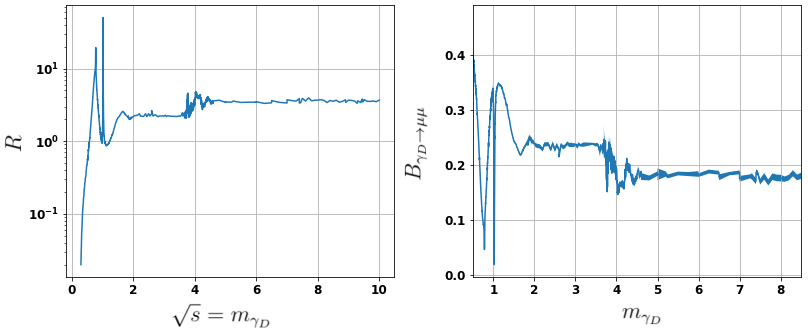
\includegraphics[width=0.95\textwidth]{Cap1/imagenes/probabilidad.png}
    \caption{Valores de $R$ (izquierda) y de probabilidad $B_{\gamma_D\rightarrow \mu\mu}$ (derecha) con el valores teóricos de masa del fotón oscuro.}
    \label{probabilidades}
\end{figure}

\begin{table}[!ht]
  \begin{center}
    \scriptsize
    \begin{tabular}{|l|ccccc|} % <-- Alignments: 1st column left, 2nd middle and 3rd right, with vertical lines in between
		\toprule
		$m_{\gamma_D}$ & 0.5 GeV & 1 GeV & 2 GeV & 3 GeV & 4 GeV \\
		\midrule
		$B_{\gamma_D\rightarrow \mu\mu}$ & $0.4021 \pm 0.0023$ & $0.301 \pm 0.012$ & $0.239 \pm 0.004$ & $0.2375 \pm 0.0028$ & $0.1938 \pm 0.0053$\\
		\bottomrule
		\toprule
		$m_{\gamma_D}$ ~ $\mathbf{(GeV})$ & 5 GeV & 6 GeV & 7 GeV & 8 GeV & 8.5 GeV\\
		\midrule
		$B_{\gamma_D\rightarrow \mu\mu}$ & $0.1845 \pm 0.0041$ & $0.1818 \pm 0.00331$ & $0.1869 \pm 0.0035$ & $0.1764 \pm 0.0061$ & $0.1805 \pm 0.0055$\\
       	%$\Gamma_{\gamma_D} ~ \mathbf{(MeV)}$ & 1 & 1.2 & 1.9 & 2.1 & 11.4 & 8.0 & 15.5 & 20.3 & 114.6 \\
       	%\midrule
       	%$f(m_{\gamma_D}) ~ \mathbf{(GeV^{-1})}$ & 952.9 & 817.2 & 538.9 & 480.2 & 87.4 & 125.1 & 64.6 & 49.2 & 8.7 \\
      	\bottomrule    
    \end{tabular}
    \caption{Probabilidades de descomposición del fotón oscuro $\gamma_D$ a par de muones.}
    \label{an-15-455:tb1}
  \end{center}
\end{table}

Las expresiones para los anchos parciales permiten el cálculo del tiempo de vida del fotón oscuro:
\begin{eqnarray}
\label{an-15-455:ec6}
\tau_{\gamma_D} = \dfrac{1}{\Gamma_{\gamma_D}} =\dfrac{1}{\Gamma_{\gamma_D \rightarrow e^+ e^-} + \Gamma_{\gamma_D \rightarrow \mu^+ \mu^-} + \Gamma_{\gamma_D \rightarrow \mathbf{hadrones}}}
\end{eqnarray}
El tiempo de vida está directamente relacionada con el parámetro $\epsilon$ y la masa del fotón oscuro se obtiene:
\begin{eqnarray}
\label{an-15-455:ec7}
\tau_{\gamma_D}(\epsilon,m_{\gamma_D}) =\dfrac{f(m_{\gamma_D})}{\epsilon^2} 
\end{eqnarray}
Es conveniente representar el tiempo de vida $\tau_{\gamma_D}$ en unidades de distancia $c\tau_{\gamma_D}$, donde $c$ es la velocidad de la luz. %También es conveniente medir $c\tau_{\gamma_D}$ en milímetros porque la sensibilidad del análisis a esta variable es $\sigma(mm)$. 
Las restricciones sobre $\epsilon$ y la masa del fotón oscuro podrían obtenerse a partir de las restricciones sobre el tiempo de vida del fotón oscuro porque están directamente relacionadas entre sí como se ve en las expresiones anteriores.

%Figura 4: Izquierda: Ancho total considerando los diferentes modos de desintegración del fotón oscuro, normalizado por e2. Derecha: ¡Relación de ramificación para gD! mm modo de decaimiento. Las expresiones para los anchos parciales permiten el cálculo de la vida útil del fotón oscuro a través de:

\begin{figure}[!t]
    \centering
    (a)
    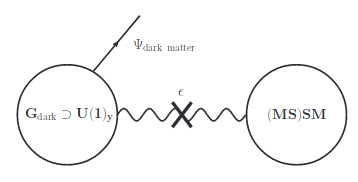
\includegraphics[width=0.55\textwidth]{Cap1/imagenes/sketch_darksector.png}
    (b)
    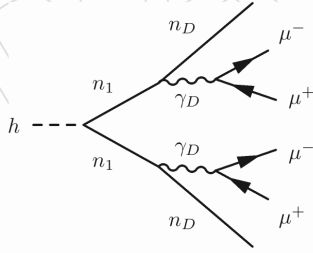
\includegraphics[width=0.35\textwidth]{Cap1/imagenes/darksusy_feynman.png}
    \caption{(a) Ilustración esquemática de la conexión entre el sector oscuro y el modelo estándar, los cuales están conectados mediante un término de mezcla dinámica. (b) Diagrama de Feynman \textbf{Dark}-\SUSY ~ del proceso vía $h \rightarrow 2n_1 \rightarrow 2n_D + 2\gamma_D \rightarrow 2n_D + 4\mu$.}
    \label{fig:sketch_darksector}
\end{figure}

La descomposición del bosón neutralino visible $n_1$ a un par de muones con carga opuesta es equivalente a $\mathcal{B}(n_1 \rightarrow 2\mu)$, con la inclusión de los modelos oscuros de \SUSY ~ que teorizan la ruptura de una nueva simetría $U(1)_D$ dando lugar el fotón oscuro masivo $\gamma_D$, el cual es dependiente de su masa $m_{\gamma_D}$ y el parámetro de mezcla cinética. Este proceso se muestra como una posible exploración de gran interés científico. El tiempo de vida corto de la partícula $\gamma_D$ no se limita a valores pequeños ya que se espera que se mantenga estable por cierto período. Por lo que es importante acomodar la posibilidad de fotones oscuros de larga duración en las búsquedas requeridas. El diagrama de Feynman \textbf{Dark}-\SUSY ~ del proceso vía $h \rightarrow 2n_1 \rightarrow 2n_D + 2\gamma_D \rightarrow 2n_D + 4\mu$ se muestra en la Fig. \ref{fig:sketch_darksector}b. Este modelo de referencia es solo un escenario posible, y se elige como una representación única de un rango muy amplio de espacio de parámetros disponibles. %Este modelo simple del sector oscuro se puede ampliar de varias maneras; versiones más complejas involucran otros bosones oscuros de Higgs, $W$ y $Z$. También hay muchos otros procesos permitidos, como por ejemplo $pp \leftarrow h \leftarrow Z_D Z / Z_D Z_D / Z_a \leftarrow 4\mu$. En este análisis representamos los resultados de una manera que permite reinterpretaciones adicionales en el marco de otros modelos.






























